\documentclass[grado3]{LEMA-Tikz-IM}

\usepackage{graphicx}  % Needed to include graphics
\usepackage{pifont} % For the scissors symbol

\begin{document}
\begin{tikzpicture}
% \pgfplotsset{compat=1.18}

% page canvas letter size
\path (0,0) rectangle (8.5in,11in);

\def\myMargin{1in}

\coordinate (botLeft) at (\myMargin,\myMargin);
\coordinate (botRight) at (8.5in-\myMargin,\myMargin);
\coordinate (topRight) at (8.5in-\myMargin,11in-\myMargin);
\coordinate (topLeft) at (\myMargin,11in-\myMargin);

% clip outside the margin 
% \draw (botLeft) rectangle (topRight);


% find center of printable page
\coordinate (centerTop) at ($ (topLeft)!0.5!(topRight) $);

% add content
\node[anchor=north, text width=6.5in] (table) at ([yshift=-1in]centerTop) {%
    \begin{enumerate}
    \item Hazle preguntas a tu compañero sobre sus hechos de multiplicación. Clasifica los hechos de tu compañero en una de estas columnas:

    \vspace{0.5cm}
    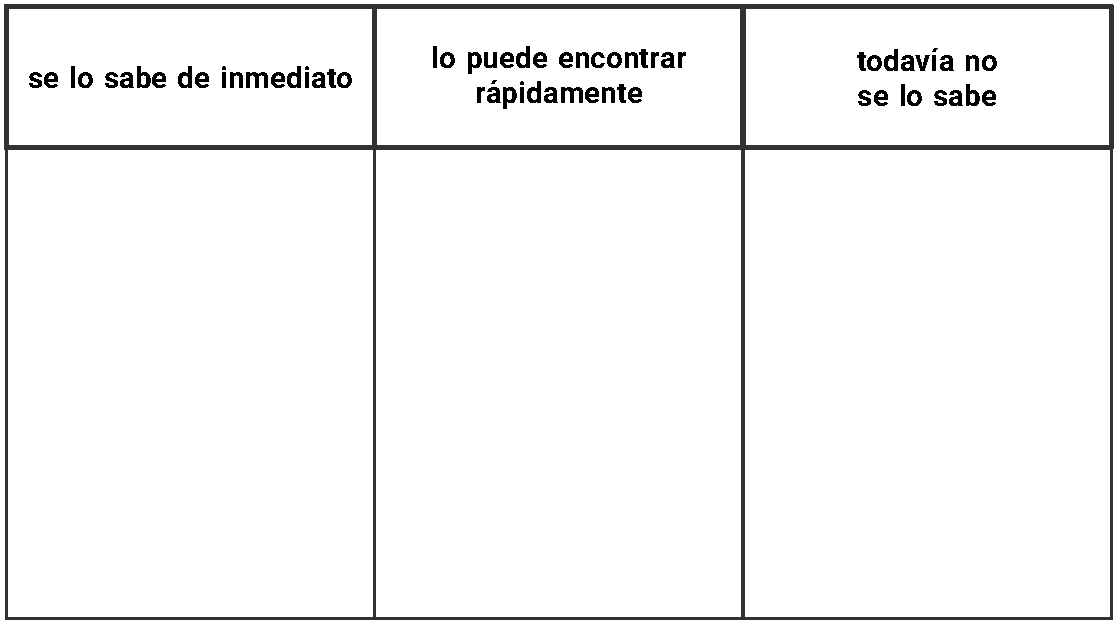
\includegraphics{../../tikz-source/clasificacionTarjetas-mult-paraBLM.pdf}
    \vspace{0.5cm}
    \item Anota cinco expresiones de multiplicación que vas a practicar.
        \begin{enumerate}%[itemsep=2ex]
            \item \vspace*{2ex}
            \item \vspace*{3ex}
            \item \vspace*{3ex}
            \item \vspace*{3ex}
            \item \vspace*{3ex}
        \end{enumerate}
    \end{enumerate}
};


% Add BLM heading to top and bottom
\node[below right, font=\bf\LARGE] (titulo) at (topLeft) {Clasificación de tarjetas: Multiplicación};
\node[font=\bf\large, below = 0.2ex of titulo.south west, anchor=north west] (subtitulo) {Hoja de registro};


% Espacio de nombre
% \node[below left] at ([yshift=-6ex]topRight) {Nombre: \underline{\hspace{6cm}}};




\end{tikzpicture}
\end{document}